\chapter{Generátor zvuků}
Zvukový generátor je důležitou součástí \zkratka{LG} vesty. Zajišťuje generování zvuků, jejichž stěžejním cílem je informování hráčů o aktuálním dělení v aréně a také zlepšují výsledný prožitek ze hry.

\section{Požadavky na generátor}
Pro generátor je jedním z nejdůležitějších požadavků jeho paměť alespoň 800~\jedn{kB}, aby se do ní vešli všechny vzorky zvuků i firmware.  možnost jej řídit pomocí \zkratka{UART} a jednoduchá indikace přehrávání a možnost snížit odběr generátoru pomocí GPIO.

%\section{Převody ADC DAC}
%TODO


\section{Realizace generátoru}
\begin{figure}[H]
    \begin{center}
        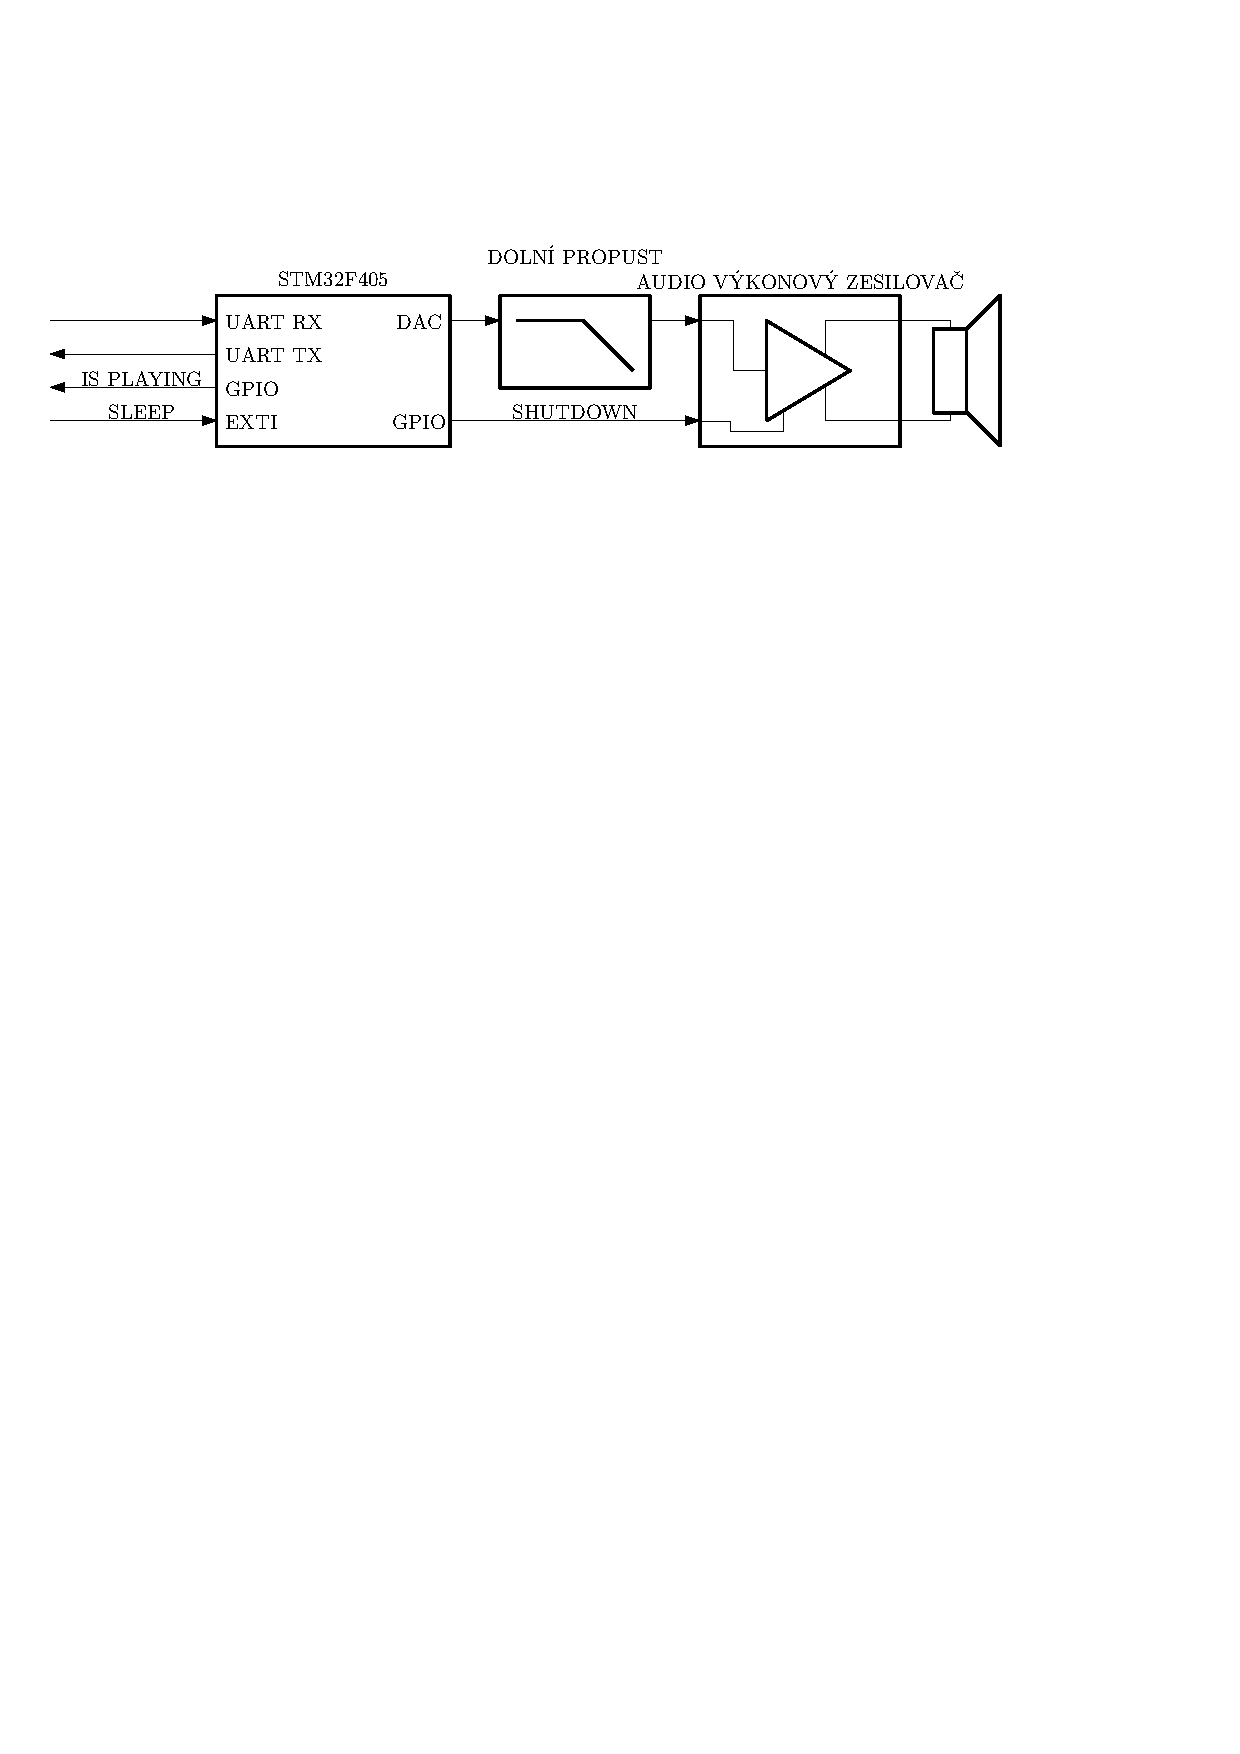
\includegraphics[width=\textwidth]{img/sound-system}
    \end{center}
    \caption{blokové znázornění zvukového generátoru}
\end{figure}

Generátor je založen na mikroprocesoru STM32F405, který je vybavený 1~\jedn{MB} paměti FLASH, která je využita, z velké části, k uložení vzorků zvuků. Ve zbytku paměti je uložen firmware generátoru. Výše zmíněný mikroprocesor, také obsahuje mimo jiné 12~\jedn{b} DAC, až 32\jedn~{b} čítače / časovače, DMA, či
UART.

Zvuky jsou v paměti reprezentovány vzorky. Tedy polem kvantovaných hodnot snímaných v diskrétních časech, které popisují zvukové vlny.

Pokud chceme obnovit původní signál, je třeba tyto vzorky signálu ve stejných časech převádět pomocí DAC na napětí. K tomu je využita jednotka DMA a časovač. DMA je nakonfigurováno tak, aby přenášelo vzorky vybraného zvuku z paměti FLASH do DAC. Jednotka DAC je přitom spouštěna časovačem, který generuje spouštěcí signál stejnou frekvencí jako byla vzorkovací frekvence zvuků, tedy 16~\jedn{kHz}. Na výstupu mikroprocesoru tedy můžeme pozorovat napětí odpovídající hodnotám vzorků.

Následně je třeba signál obnovit pomocí rekonstrukčního (anti-aliasingového) filtru, tedy filtru typu dolní propust. Ten ze signálu odstraní nežádoucí spektrální složky, které vznikají skoky z hodnoty jednoho vzorku na vzorek druhý. Filtr byl navržen pomocý online návrhového prostředí firmy Analog Devices.

Poté je signál zesílen ve výkonovém integrovaném audio zesilovači LM4861 a přiveden do reproduktoru, kde dojde k jeho převodu na akustický signál.

\section{Komunikační protokol}
S generátorem se jednoduše komunikuje pomocí UARTu. Během komunikace se rozlišuje mezi třemi typy příkazů:
\begin{itemize}
    \item zastavit přehrávání
    \item změnit zvukovou sadu
    \item přehrát zvuk z nastavené zvukové sady (skupiny zvuků namluvené stejným jazykem)
\end{itemize}


\begin{table}[H]
  \caption{Kompletní seznam příkazů zvukového generátoru}
  \begin{center}
  	\small
	  \begin{tabular}{|l|r|}
	    \hline
	    \textbf{název} & \textbf{kód} \\\hline\hline
        \texttt{SOUND\_CMD\_STOP}                 &  0 \\\hline
        \texttt{SOUND\_CMD\_SET\_SOUND\_SET\_EN}  &  1 \\\hline
        \texttt{SOUND\_CMD\_SET\_SOUND\_SET\_CZ}  &  2 \\\hline
        \texttt{SOUND\_CMD\_PLAY\_ACTIVATED}      &  3 \\\hline
        \texttt{SOUND\_CMD\_PLAY\_GUN}            &  4 \\\hline
        \texttt{SOUND\_CMD\_PLAY\_DONT\_GIVE\_UP} &  5 \\\hline
        \texttt{SOUND\_CMD\_PLAY\_GAME\_OVER}     &  6 \\\hline
        \texttt{SOUND\_CMD\_PLAY\_GO}             &  7 \\\hline
        \texttt{SOUND\_CMD\_PLAY\_KEEP\_GOING}    &  8 \\\hline
        \texttt{SOUND\_CMD\_PLAY\_NUMBER\_1}      &  9 \\\hline
        \texttt{SOUND\_CMD\_PLAY\_NUMBER\_2}      & 10 \\\hline
        \texttt{SOUND\_CMD\_PLAY\_NUMBER\_3}      & 11 \\\hline
        \texttt{SOUND\_CMD\_PLAY\_NUMBER\_4}      & 12 \\\hline
        \texttt{SOUND\_CMD\_PLAY\_NUMBER\_5}      & 13 \\\hline
        \texttt{SOUND\_CMD\_PLAY\_PLAY}           & 14 \\\hline
        \texttt{SOUND\_CMD\_PLAY\_WELL\_DONE}     & 15 \\\hline
	  \end{tabular}
  \end{center}
\end{table}
